\chapter{Training \glsxtrlong{marl} Policies for Quadrotors with Payload}

This chapter presents our methodology for training decentralized \gls{marl} policies that enable a team of Crazyflie quadrotors to cooperatively transport a cable-suspended payload. We begin by formulating the cooperative transport task as a \gls{dec-pomdp}, defining the state, action, and observation structures. We then describe our high-performance simulation and training pipeline, and finally present the modular reward design used to train our policies.
\section{Problem Formulation}

We model a team of $Q$ Crazyflie quadrotors collaboratively carrying a cable-suspended payload as the \gls{dec-pomdp} $(\mathcal{Q}, \mathcal{S}, \{\mathcal{A}^i\}_{i=1}^Q, P, r, \{\Omega^i\}_{i=1}^Q, O, \rho_0, \gamma)$, where $\mathcal{Q} = \{1,2,\dots,Q\}$ is the set of agents. At each discrete timestep $t$, the global state 
\begin{equation}
s_t = \bigl(\{\mathbf{p}^i_t,\mathbf{v}^i_t,\mathbf{R}^i_t,\boldsymbol{\omega}^i_t\}_{i=1}^Q,\; \mathbf{p}^P_t,\mathbf{v}^P_t\bigr)
\end{equation}
encapsulates each quadrotor's position $\mathbf{p}^i_t \in \mathbb{R}^3$, velocity $\mathbf{v}^i_t \in \mathbb{R}^3$, attitude $\mathbf{R}^i_t \in SO(3)$, angular velocity $\boldsymbol{\omega}^i_t \in \mathbb{R}^3$, and the payload's position $\mathbf{p}^P_t \in \mathbb{R}^3$ and velocity $\mathbf{v}^P_t \in \mathbb{R}^3$. The transition model $P(s_{t+1}\mid s_t, a_t)$ corresponds to a single simulation step in MuJoCo MJX, which approximates the continuous quadrotor and payload dynamics (including cables) over the fixed interval $\Delta t$.

The initial state is sampled from a distribution $\rho_0$. In our case $\rho_0$ defines harsh initial conditions, such that the policies must learn to recover from them.

Each agent $i$ selects an action 
\begin{equation}
a^i_t = (f^i_{1,t},f^i_{2,t},f^i_{3,t},f^i_{4,t}) \in \mathbb{R}^4
\end{equation}
where $f^i_{j,t}$ is the thrust of rotor~$j$. The joint action of all agents is $a_t = (a^1_t,\dots,a^Q_t)$. 

We define the payload position tracking error as
$
\mathbf{e}^P_t = \mathbf{p}^P_t - \mathbf{p}^P_{\mathrm{des},t},
$
so that $e^P_t = \|\mathbf{e}^P_t\|$ represents the tracking error at time $t$. The main objective is to minimize this error while maintaining stability in the system. This gives us a rough reward structure of:
\begin{equation}
r(s_t,a_t) \approx\; - e^P_t \;-\; \text{(stability penalties)}
\end{equation}
We penalize payload tracking error and include additional terms to discourage large payload swing or cable-tension imbalance.

Each agent must observe its own state as well as the payload's state and the position of the other agents to be able to avoid them. Therefore agent $i$ observes
\begin{equation}
    \label{eq:obs}
    \tilde{o}^i_t 
    = \Bigl(
      \hat{\mathbf{p}}^i_t,\;
      \hat{\mathbf{v}}^i_t,\;
      \hat{\mathbf{R}}^i_t,\;
      \hat{\boldsymbol{\omega}}^i_t,\;
      \mathbf{e}^P_t,\;
      \mathbf{v}^P_t,\;
      \{\hat{\mathbf{p}}^j_t\}_{j \in \mathcal{Q}\setminus\{i\}}
    \Bigr).
\end{equation}
\emph{Note that \(\tilde{o}^i_t\) is a simplified observation. The exact observation model is defined below.}

where $\hat{\mathbf{p}}^i_t,\hat{\mathbf{v}}^i_t,\hat{\mathbf{R}}^i_t,\hat{\boldsymbol{\omega}}^i_t$ are \gls{ekf} estimates of its own state and $\mathbf{e}^P_t,\mathbf{v}^P_t$ are the payload state from \gls{mocap}. To reduce notational complexity we will denote the observation component without $\hat{\cdot}$ as $\mathbf{p}^i_t,\mathbf{v}^i_t,\mathbf{R}^i_t,\boldsymbol{\omega}^i_t$. The observation function $O(o^i_t \mid s_t)$ models sensor noise and maps the global state $s_t$ to each $o^i_t$. Finally, $\gamma \in [0,1)$ is the discount factor.

Agents share a single policy conditioned on their current observation \(o^i_t\) and the previous action \(a^i_{t-1}\) and parameterized by \(\theta\). The actions are sampled as
\begin{equation}
  a^i_t \sim \pi_{\theta}\bigl(a^i_t \mid o^i_t,\;a^i_{t-1}\bigr)
  \quad\text{for }i=1,\dots,Q.
\end{equation}


For multiple agent scenarios we sample the actions independently for each agent, so that the joint action is given by $a_t = \bigl(a^1_t,\dots,a^Q_t\bigr)$.


We seek the shared parameters \(\theta\) that maximize the expected discounted return
\begin{equation}
\begin{aligned}
\text{maximize}\quad & J(\theta) = \mathbb{E}\Bigl[\sum_{t=0}^\infty \gamma^t\,r(s_t,a_t)\Bigr],\\
\text{subject to}\quad &s_0 \sim \rho_0,\\
&s_{t+1} \sim P\bigl(\cdot\mid s_t,a_t\bigr),\\
&o^i_t \sim O\bigl(\cdot\mid s_t\bigr),\\
&a^i_t \sim \pi_{\theta}\bigl(\cdot\mid o^i_t,a^i_{t-1}\bigr)
\quad\forall i.
\end{aligned}
\end{equation}
By maximizing \(J(\theta)\), the agents learn to jointly minimize payload tracking error \(e^P_t\) while maintaining stability throughout the cooperative transport task.

We have now formalized the problem as a \gls{dec-pomdp}, which allows us to apply decentralized \gls{marl} algorithms to learn policies that can handle the complexities of multi-agent coordination in cable-suspended payload transport tasks. The next section describes the CrazyMARL framework, which provides the necessary simulation and training infrastructure to implement this efficiently.
\todo{maybe add fig wit multiple agents and env...}

\section{CrazyMARL}
We present \textbf{CrazyMARL}, an end-to-end JAX-based pipeline for training \gls{marl} policies on teams of Crazyflie quadrotors. Our extendable framework implements both learning for a single quadrotor without payload, as well as single-vehicle and cooperative multi-agent cable-suspended payload transport tasks. At its core, the simulation leverages the high-performance MJX backend of the MuJoCo physics engine \cite{todorov_mujoco_2012}, interfaced through the Brax library for highly parallelized training. Our environments and algorithms are based on JaxMARL introduced by \autocite{flair2023jaxmarl}. We expose the simulator as a \texttt{JAXMARL.Mabrax} environment, providing a drop-in \gls{api} for JAX-based RL algorithms and other research algorithm implementing the JaxMARL api.

\subsection{Simulation Environment}

Our framework provides a configurable environment generator for simulating multi-agent cable-suspended payload transport tasks, as well as swarm control of single quadrotors. The environment is designed to be modular and extensible, allowing for easy definition of new scenarios. The environment can be initialized with a configuration, defining the number of quadrotors, the payload mass, cable length, and other parameters. The environment supports both single-agent and multi-agent scenarios, where each agent is a quadrotor with its own observations and actions.
\begin{figure}
\centering
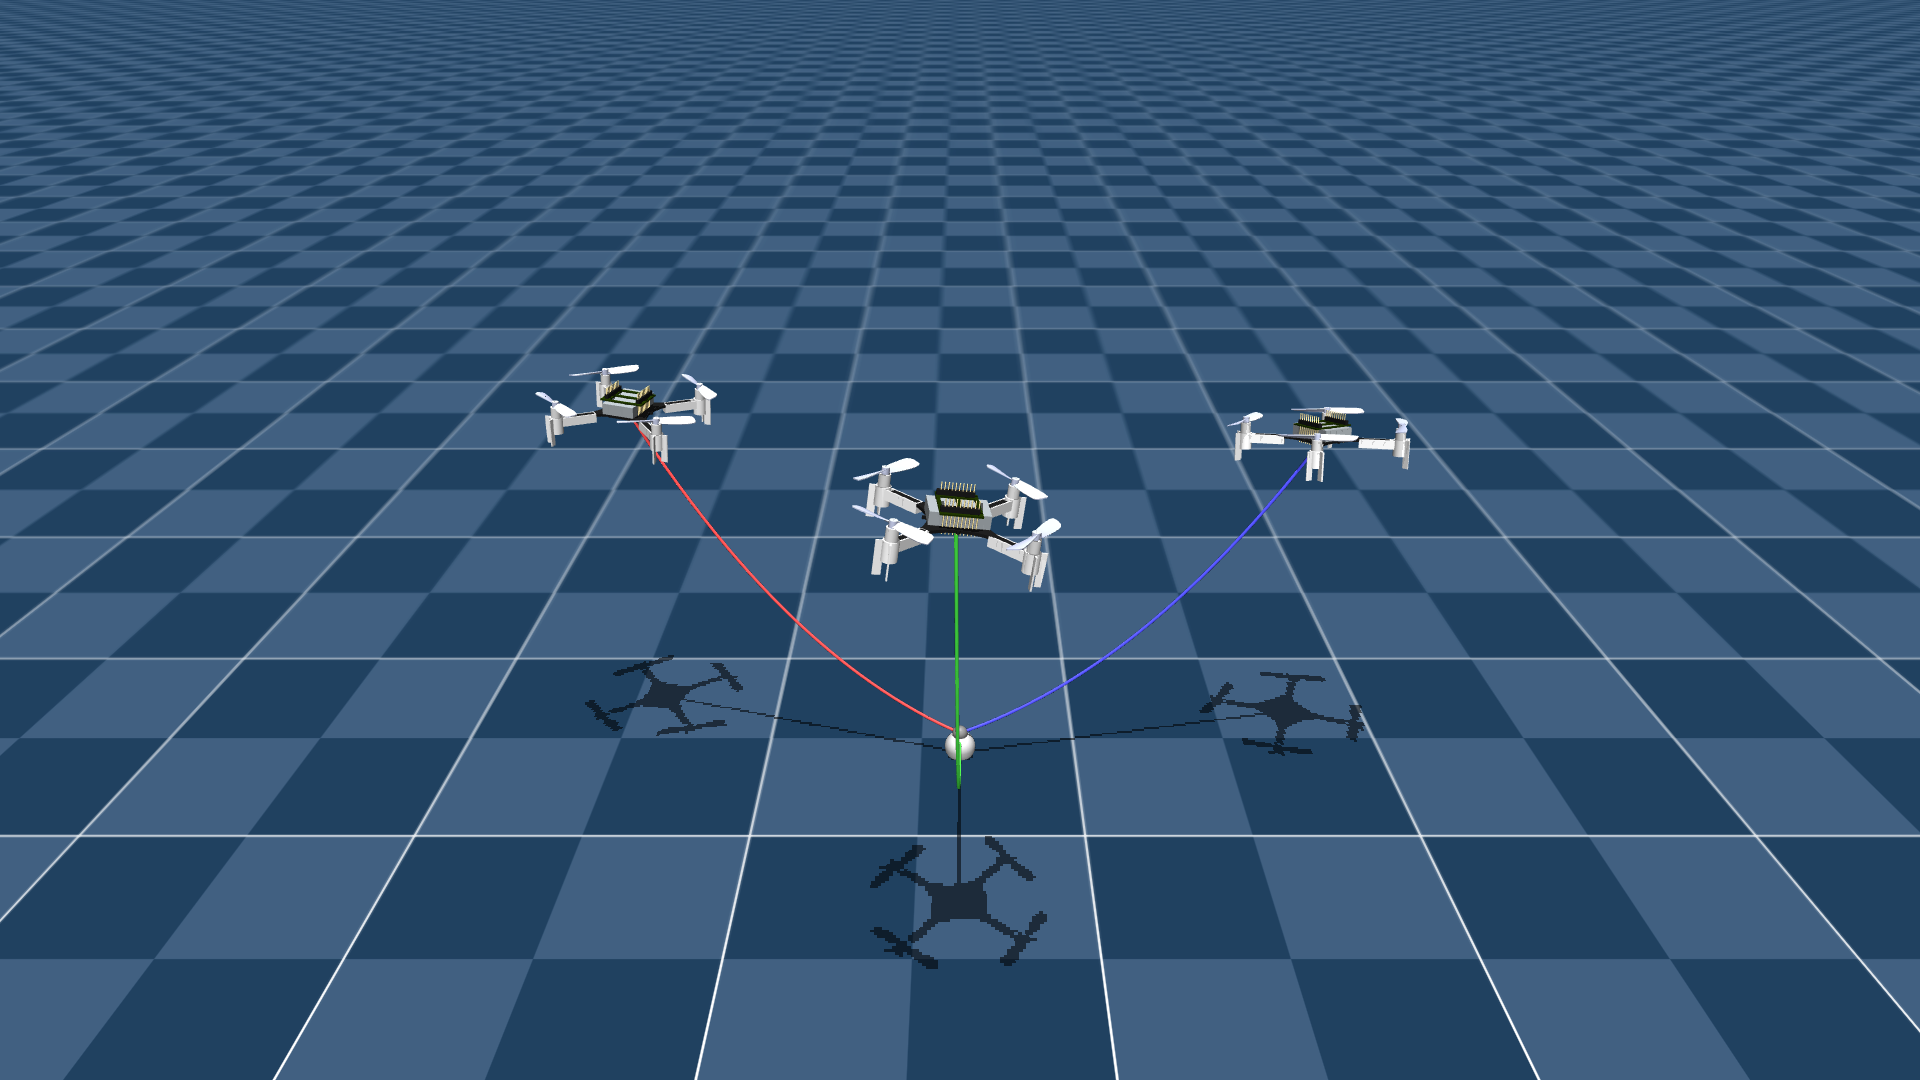
\includegraphics[width=0.6\textwidth]{figs/quad_env.png}
\caption[Simulation Environment]{Rendering of the MuJoCo simulation with three quadrotors carrying a cable-suspended payload.}
\label{fig:crazyflie_env}
\end{figure}

Figure~\ref{fig:crazyflie_env} shows a rendering of the simulation environment with three quadrotors carrying a cable-suspended payload. The environment is built upon the MuJoCo physics engine, which provides accurate and efficient simulation of rigid body dynamics, including contact and friction. The MJX solver is used to compute the physics updates in parallel on the GPU, allowing for high-performance training of \gls{rl} policies with up to 32k parallel environments. We can also visualize the simulation using the rendering capabilities of MuJoCo, which provides a realistic representation of the quadrotors, payload, and cables.

The quadrotors are modeled as rigid bodies with four rotors, each producing thrust and a small torque. We optionally reduce the quadrotors collision mesh to a rectangular prism in order to speed up collision detection. The payload is modeled as a rigid body sphere suspended by cables, which are represented as tendons in MuJoCo. The shape and attachment points of the payload are configurable. The cables connect the quadrotors to the payload and can be configured with different lengths and properties. The environment also supports obstacles, which were not yet further utilized in our work, but could be a good basis for future work on obstacle avoidance or dynamic interactions with the environment.

We implement the JaxMARL \gls{api} for multi agent environments based on Gymnax \autocite{gymnax2022github}. This wraps our environment in a standardized interface that can be used with any compatible \gls{rl} algorithm. The wrapper adds an abstraction layer to the simulation. Each timestep we call a step function with a set of actions for each quadrotor and the environment returns the updated state which is then used to compute the rewards and observations for each agent.

\subsection{Observation Mapping}
In practice we slightly adjust the observation structure defined in Equation~\eqref{eq:obs}. Each agent \(i\) still receives a local observation vector \(\mathbf{o}^i_t\) that contains its own state, the payload's state, and the relative positions of other agents.  This ensures that each agent can act based on its own measurements and the shared payload information, while not directly observing other agents' internal states. To define the observation space, we first define the global observation vector \(\mathbf{o}_t\) that contains all relevant information about the system state at time \(t\). This also serves as the basis for computing rewards and termination conditions and allows for a centralized training setup.
\subsubsection{Global Observations}
At each control step \(t\), the simulation environment produces a high-dimensional state vector. We map this to a global observation vector 
\begin{equation}
\mathbf{o}_t \;=\; \bigl[\;\underbrace{\mathbf{e}^P_t}_{3},\;\underbrace{\mathbf{v}^P_t}_{3},\;\underbrace{\{\;\mathbf{r}^i_t,\;\mathrm{vec}(\mathbf{R}^i_t),\;\mathbf{v}^i_t,\;\boldsymbol{\omega}^i_t,\;\mathbf{a}^i_t\}_{i=1}^Q}_{Q(3+9+3+3+4)}\bigr] \;\in\;\mathbb{R}^{6 + 22Q}
\end{equation}
Here \(\mathbf{e}^P_t = (\mathbf{p}^P_{\mathrm{des},t}-\mathbf{p}^P_t)/\max(\|\mathbf{p}^P_{\mathrm{des},t}-\mathbf{p}^P_t\|,1)\) is the normalized payload tracking error and \(\mathbf{v}^P_t\) its velocity. Giving the error as observation instead of an absolute position, allows us to give a position setpoint and track trajectories. We normalize the error to have the policy automatically generalize to a target at any distance. For each quadrotor \(i\), \(\mathbf{r}^i_t=\mathbf{p}^i_t-\mathbf{p}^P_t\) denotes its position relative to the payload, \(\mathrm{vec}(R^i_t)\in\mathbb{R}^9\) the row-major flattening of its rotation matrix, \(\mathbf{v}^i_t\) is the linear velocity in world frame, \(\boldsymbol{\omega}^i_t\) its body-frame angular velocities and \(\mathbf{a}^i_{t-1}\) the agents previous action. By construction, this global observation vector contains all information required to compute rewards and termination conditions. It can be easily adjusted to include additional information or other mappings.

\subsubsection{Local Observations}
Since we want to train our policy in a \gls{ctde} fashion, we map the global observation vector to each agent's local observation space. During decentralized execution, each agent \(i\) receives only the subset of entries corresponding to the payload terms, its own dynamic state block, and the other quadrotors relative positions.  Concretely, agent \(i\) observes
\begin{equation}
\mathbf{o}^i_t 
\;=\;
\bigl[\,
\mathbf{e}^P_t,\;\mathbf{v}^P_t,\;\mathbf{r}^i_t,\;\mathrm{vec}(\mathbf{R}^i_t),\;\mathbf{v}^i_t,\;\boldsymbol{\omega}^i_t,\;\mathbf{a}^i_{t-1},\;
\{\mathbf{r}^j_t\}_{j \in \mathcal{Q}\setminus\{i\}}
\,\bigr]\;\in\;\mathbb{R}^{6 + 22 + Q - 1}\,,
\end{equation}
so that each policy conditions on the payload's error and velocity, the agent's full pose and velocity, and its previous action. This restriction enforces the \gls{dec-pomdp} structure, by hiding other agents' internal states, coordination must emerge through the shared reward alone.

The observation structure can also be used for a scenario without a payload, where the team observations containing payload position and velocity are omitted.
\subsubsection{Observation Noise}
To account for sensor imperfections, we can inject structured Gaussian noise into the global observation vector at each timestep. Concretely, given an observation $\mathbf{o}$, we draw a standard normal vector $\bm{\eta}\sim\mathcal{N}(\mathbf{0},\mathbf{I})$ of the same dimension and compute
\begin{equation}
    \mathbf{o}' = \mathbf{o} + \sigma_{\mathrm{obs}}\,\bm{\Lambda}\,\bm{\eta}\,,
\end{equation}
where $\sigma_{\mathrm{obs}}$ is a tunable noise amplitude and $\bm{\Lambda}\in\mathbb{R}^{6+22Q}$ is a diagonal scaling vector to tune the noise level for each observation component. We chose each scale factor by examining the typical range of values for its corresponding observation component and setting the noise magnitude accordingly. This ensures that each component of the observation is corrupted by noise proportional both to its typical magnitude and the global noise level.
\subsection{Action Space}
The policy of each agent \(i\) outputs a four-dimensional vector \(\mathbf{a}^i_t\in[-1,1]^4\), representing normalized thrust commands for its rotors. By adopting the \gls{srt} model, we retain the full dynamic fidelity of the quadrotor, enabling capable agile maneuvers.
 These are mapped to physical rotor forces via
\begin{equation}
f^i_{j,t}
\;=\;
\frac{a^i_{j,t} + 1}{2}\;f_{\max}^i,
\qquad
j=1,\dots,4,
\end{equation}
where \(f_{\max}^i\) is the agent-specific maximum thrust, randomly perturbed at the start of each episode to improve robustness.  Optionally, zero-mean Gaussian noise proportional to \(f_{\max}^i\) may be added to each \(f^i_{j,t}\) to model actuator uncertainty. We always constrain \(\mathbf{a}^i_t\in[-1,1]^4\) and sample \(f_{\max}^i\) within a known bound to produce safe thrust profiles. The resulting thrust vector \(\mathbf{f}^i_t\) is then applied in the physics simulator with the proportional torque component.
\todo{maybe talk about the motor delay model...}
\subsection{Randomization}
To train a robust policy that can handle a wide range of initial conditions and disturbances, we apply several randomization techniques during training.
\subsubsection{Initial-State Randomization}
\label{sec:reset}
\begin{figure}
    \centering
    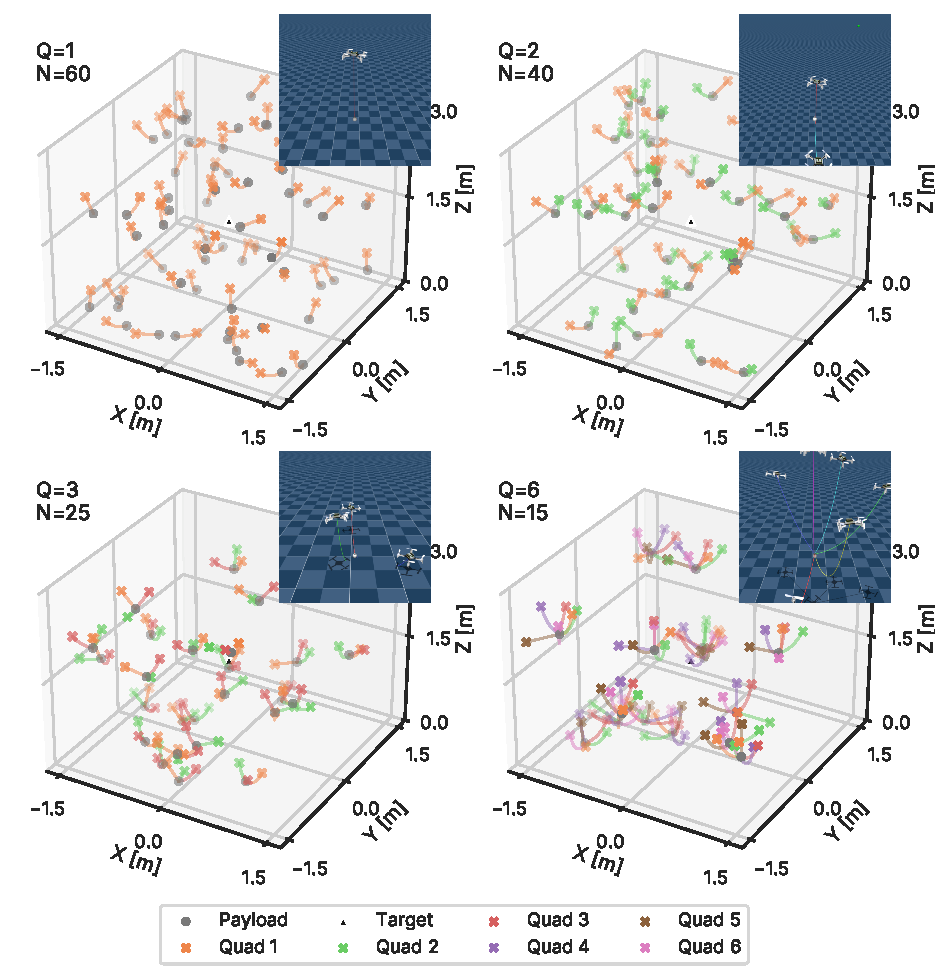
\includegraphics[width=\textwidth]{experiments/initial_states.pdf}
    \caption[Initial States]{Randomly sampled initial configurations for the payload and quadrotors. We show configurations for Q = 1, 2, 3 and 6 quadrotors. For visualization purposes we reduce the number of different runs (N) visualized. Here the payload position is sampled uniformly without target bias. The payload is positioned at the center of each configuration, while quadrotors are uniformly distributed in a spherical shell around it. A lot of configurations start with slack cables. Some configurations start on the ground.}
    \label{fig:reset_config}
\end{figure}
A key aspect of our approach is the initial-state randomization $s_0\sim\rho_0$, which generates diverse initial configurations for the payload and quadrotors. This helps the policy learn to handle a wide range of challenging scenarios, including starting from the ground, hovering, disturbance rejection, modeswitch of the payload cable and strong payload swing. The initial conditions are sampled at each reset of the environment, ensuring that the policy is exposed to a variety of situations during training. This is crucial for learning robust behaviors. 
At each reset, the payload center~$p$ is sampled uniformly around the target at $[0,0,1.5]$ in
\begin{equation}
p^P_{xy}\sim\mathcal{U}([-1.5,1.5]),\quad p^P_z\sim\mathcal{U}([-1,3]),
\end{equation}
where the $z$-coordinate is clipped to ensure the payload is above the ground, allowing us to adjust the ratio of ground-takeoff starting positions. We additionally add a subset initializations near the payload with $p^P\sim\mathcal{N}(\mathbf{0},0.02\mathbf{I})$. This ratio of target initializations is usually set to 20\% in training to help with learning accurate tracking.

We can then use the payload position $p^P$ as the center point and randomly sample $N$ quadrotors in a spherical shell around the payload. The radius $r_i$ of each quadrotor is sampled from a normal distribution with mean $\mu_r$ and standard deviation $\sigma_r$, and then clipped to cable length. The angles $\theta_i$ and $\phi_i$ are sampled from normal distributions with means $\mu_\theta$ and $\phi_{\mathrm{offset}}$ respectively, and standard deviations $\sigma_\theta$ and $\sigma_\phi$. The angles are then adjusted to ensure they are within the range $[0, 2\pi]$. The equations for sampling the quadrotor positions are as follows:
\begin{equation}
r_i = \mathrm{clip}\bigl(\mu_r+\sigma_r\varepsilon_i^{(r)},\,r_{\min},\,r_{\max}\bigr),\quad
\theta_i = \mu_\theta+\sigma_\theta\varepsilon_i^{(\theta)},\quad
\phi_i = \tfrac{2\pi(i-1)}{Q} + \phi_{\mathrm{offset}} + \sigma_\phi\varepsilon_i^{(\phi)},
\end{equation}
where we found these parameters to work well in practice across the different number of quadrotors. $c$ is the length of the cable, which is also the maximum radius for the quadrotors.
\begin{equation}
\begin{aligned}
\varepsilon_i^{(r)},\,\varepsilon_i^{(\theta)},\,\varepsilon_i^{(\phi)}
    &\sim \mathcal{N}(0,1), \quad
\phi_{\mathrm{offset}} \sim \mathcal{U}(-\pi,\pi),\\
\mu_r &= c,\quad
\sigma_r = \tfrac{c}{3},\quad
r_{\min} = 0.05,\quad
r_{\max} = c,\\
\mu_\theta &= \tfrac{\pi}{7},\quad
\sigma_\theta = \tfrac{\pi}{8},\quad
\sigma_\phi = \tfrac{\pi}{N+1}\,.
\end{aligned}
\end{equation}

These are converted to Cartesian positions with the $z$-coordinate clipped.
\begin{equation}
q_i = p + r_i
\begin{bmatrix}
\sin\theta_i\cos\phi_i\\
\sin\theta_i\sin\phi_i\\
\cos\theta_i
\end{bmatrix},
\end{equation}
We oversample configurations with this strategy and filter out all configurations where the quadrotors are initially in collision. This results in a even distribution of valid initial configurations with some very harsh initial conditions for any number of quadrotors as shown in \autoref{fig:reset_config}. This also includes starting from the ground. 

We also randomize the quadrotor attitude. Roll and pitch angles are drawn from $\mathcal{N}(0,10^\circ)$ and clipped to $\pm90^\circ$, while yaw is sampled uniformly from $[-180^\circ,180^\circ]$.

Each component of the linear velocity vector $\mathbf{v}$ is sampled from a zero-mean Gaussian with a standard deviation of $0.2\,m/s$. Each component of the angular velocity (body-rate) vector $\boldsymbol{\omega}$ is sampled similarly with a standard deviation of $20^\circ/s$.

This creates a wide range of initial conditions, including starting from the ground, hovering, and various disturbances. A lot of them are very challenging to recover from. The policy must learn this recovery behavior. The Gaussian shaping of the randomization parameters is chosen to ensure that there are also sufficient easier initial conditions, such that the policy can learn the basic hover behavior.
\subsubsection{Domain Randomization}
To further improve robustness, we apply domain randomization techniques during training. For most experiments we focus on randomizing the quadrotor's maximum thrust $f_{\max}^i$ within a range of $[0.8,1.0]$ times the nominal value, with some small Gaussian offset for each motor. This not only ensures that the policy can adapt to variations in the quadrotor's  battery level and motor performance, but also brings a certain level of generalization to payload and quadrotor mass.

We also provide the option to randomize the payload mass, cable length, and other parameters, but these were not used in our experiments, since recent work \cite{eschmann_learning_2024-1} has shown that zero-shot transfer without domain randomization is possible for the Crazyflie platform. Future work could explore the impact of these additional randomizations on policy robustness, generalization and sim-to-real transfer.




\subsection{Reward Design}
A key aspect of our approach is a modular reward design for multiple quadrotors with and without cable suspended payloads.
We initially replicated reward structures from prior work for single quadrotors and swarms of quadrotors. The usual reward structure is a tracking reward penalizing or rewarding the distance to the target and varying terms to encourage learning of stable flight. The most common ones an attitude reward component and an angular velocity and linear velocity penalty. Depending on application this is also extended with a collision penalty and other auxilary reward terms \cite{molchanov_sim--multi-real_2019,eschmann_learning_2024-1,kaufmann_benchmark_2022, huang_collision_2024}.

Through an iterative process, experimenting with different extensions of these core terms, we found a very effective reward structure. The final reward structure is modular, allowing for easy adjustments and extensions. It consists of several components that encourage the desired behaviors in the quadrotors while maintaining a stable formation and effectively transporting the payload.
The goal of our reward is to encourage flight behaviors that recover the cable-suspended payload to its target at a safe speed, while simultaneously minimizing payload swing and vehicle tilt, maintaining a taut suspension cable, enforcing safe spacing between quadrotors, and promoting gentle, low-frequency thrust commands for robust sim-to-real transfer. 

Harsh penalties can induce learning-to-terminate behaviors or unstable gradients. In order to prevent this, we shape our unbounded errors inside a smooth bounded envelope with the exponential function instead of penalties. This is a common reward shaping technique in \gls{rl}, already applied in work on single quadrotors like \cite{kaufmann_champion-level_2023}.
\begin{equation}
\Phi_s(x) = \exp\bigl(-s\,\lvert x\rvert\bigr),
\qquad
\Phi(x) = \Phi_2(x).
\end{equation}
 This keeps the magnitude bounded, and makes the derivative taper off rather than spike. Figure~\ref{fig:reward_details} visualizes this function, showing how it rewards values close to zero. Here $s$ is a scaling factor that determines the steepness of the exponential decay. This function is bounded between $0$ and $1$, ensuring that the reward remains positive and bounded. This function has a strong peak at 1, decaying rapidly. The exponential decay ensures that the reward approaches zero as the error increases, but never becomes negative. This allows us to use the same reward structure for both positive and negative errors, without introducing instability in the learning process. A major benefit of this design is, that this reduces the need of coefficient balancing in the reward function, as common in previous methods. Our reward consists of the following components:
\begin{figure}

  \centering
  \begin{subfigure}[t]{0.49\textwidth}
    \centering
    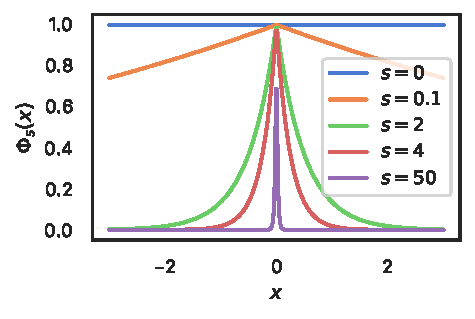
\includegraphics[width=0.96\textwidth]{figs/phi.pdf}
    \caption{}
  \end{subfigure}
  \begin{subfigure}[t]{0.49\textwidth}
    \centering
    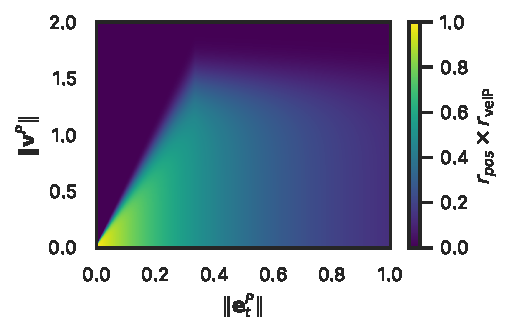
\includegraphics[width=\textwidth]{figs/reward_heatmap.pdf}
    \caption{}
  \end{subfigure}
  \caption[Reward Components]{
    (a) The reward shaping function \(\Phi_s\) used to shape reward components. The steepness factor \(s\) determines the decay rate of the function.
    (b) Plot visualization of the product of payload position and velocity reward. The reward is highest when the payload is close to the target and has very low velocity. A maximum velocity of 1.5m/s is encouraged.
  }
  \label{fig:reward_details}
\end{figure}
\subsubsection{Payload Position Error}
We define the payload position error \(\mathbf{e}^P = \mathbf{p}^P - \mathbf{p}^P_{\mathrm{des},t}\). The main objective is to minimize this error, so we define a payload tracking reward
\begin{equation}
r_{\mathrm{pos}} = \Phi\bigl(\|\mathbf{e}^P\|\bigr)
\end{equation}
We now add multiple auxilary reward terms to aid learing of hover and stable safe behaviors.
\subsubsection{Payload Velocity Alignment}
To guide the quadrotor to the target we add an auxilary velocity alignment reward.
\begin{equation}
\mathbf{v}_{\rm dir} =
\begin{cases}
\dfrac{\mathbf{v}^P}{\lVert \mathbf{v}^P\rVert},  v > \varepsilon,\\[4pt]
\mathbf{0},  \text{else}
\end{cases}
\quad
s_{\rm align} = \min(40\,\|\mathbf{e}^P\|,2), \quad
\mathbf{e}_{\rm dir} = \dfrac{\mathbf{e}^P}{\|\mathbf{e}^P\| + \varepsilon},
\end{equation}
\begin{equation}
r_{\rm dir} = \Phi_{s_{\rm align}}\!\Bigl(1 - \mathbf{v}_{\rm dir}\cdot\mathbf{e}_{\rm dir}\Bigr).
\end{equation}
This reward encourages the quadrotors to align their velocity with the direction of the payload error, which helps to reduce the tracking error more quickly in a straight line trajectory. We shape $\Phi$ with a steepness factor $s_{\rm align}$ that decreases closer to the target. This leads to the direction guidance being more pronounced at larger distances.

We combine this velocity guidance with the payload position error to form a combined tracking reward
\begin{equation}
r_{\mathrm{track}} =(r_{\mathrm{pos}} + r_{\rm dir})/2
\end{equation}

We then define multiple stability and safety rewards to ensure the quadrotors maintain a stable flight and avoid collisions with each other.

\subsubsection{Velocities}

To encourage the quadrotors to maintain a stable velocity, we discurage large velocities of quadrotors and the payload. We define a maximum desired velocity $v_{\max}$ for the payload and quadrotors, allowing us to define a safe velocity range for the payload and quadrotors. We shrink this range as the payload quadrotors approach the target, to ensure they slow down as they get closer. The maximum velocity is set to $v_{\max}=2\,m/s$ in our experiments. The velocity reward for the payload is defined as
\begin{equation}
r_{\mathrm{velP}}
= \exp\!\Biggl(-\biggl(\frac{\lVert \mathbf{v}^P\rVert}{\bigl(\min(3\,d,1)+0.02\bigr)\,0.75v_{\max}}\biggr)^{8}\Biggr)
\end{equation}
For the quadrotors velocity we apply the same shaping and calculate the mean over all quadrotors.
\begin{equation}
r_{\mathrm{velQ}}
= \frac{1}{Q}\sum_{i=1}^Q \exp\!\Biggl(-\biggl(\frac{\lVert \mathbf{v}^i\rVert}{\bigl(\min(3\,d,1)+0.02\bigr)\,v_{\max}}\biggr)^{8}\Biggr) 
\end{equation}
Figure~\ref{fig:reward_details} shows the interplay of the payload position and velocity reward. The product of these two rewards is essential for good tracking performance. Their combination allows the policy to learn perfect deceleration and stopping at the target, while also keeping velocities in a safe range.
\subsubsection{Yaw Rate}
We want to strongly discourage large yaw rates, as they can lead to unstable flight and payload swing. We define a yaw rate reward as
\begin{equation}
r_{yaw}
= \frac{1}{Q}\sum_{i=1}^{Q}\phi\bigl(\omega_z^i\bigr).
\end{equation}
\subsubsection{Inter-Agent Safe-Distance}
For $Q>1$ quadrotors we define a reward that encourages a safe distance between quadrotors. We take the mean of the shaped pairwise distances between all quadrotors, normalized to a maximum of 1. The reward is 0 for our minimum distance of $d_{min}= 0.15 m$, which is the minimum safe distance we want to enforce between quadrotors. We then increase reward to 1 when we reach our safe distance of $d_{safe}=0.18 m$. The reward is defined as
\begin{equation}
r_{\mathrm{dist}} =
\begin{cases}
\displaystyle
\frac{1}{Q(Q-1)} \sum_{i \neq j}
\mathrm{clip}\bigl(\dfrac{1}{d_{safe}-d_{\min}}\,\|\mathbf{p}^i - \mathbf{p}^j\| - d_{\min},\,0),\,1\bigr),
& Q > 1,\\[1.5ex]
1, & Q = 1.
\end{cases}
\end{equation}

\subsubsection{Orientation}
We calculate the tilt angle \(\theta^i\) between each quadrotors body-frame z axis and the world z axis. We take the mean over all quadrotors and apply a shaping function \(\Phi\) to discourage large roll or pitch angles that can lead to instability and payload swing. The reward is defined as
\begin{equation}
r_{\mathrm{up}}
= \frac{1}{Q}\sum_{i=1}^Q \Phi\bigl(\theta^i\bigr).
\end{equation}

\subsubsection{Taut-String Maintenance}
We want to encourage the quadrotors to keep the cables taut, to remain in control of the payload. We therefore encourage an increase of the distance of the quadrotors to the payload. Let \(d^{P,i}=\lVert\mathbf{p}^i-\mathbf{p}^P\rVert\) and \(h^i=(\mathbf{p}^i)_z-(\mathbf{p}^P)_z\). A taut cable of length \(L\) is encouraged by maximizing both terms via
\begin{equation}
r_{\mathrm{taut}}
= \frac{1}{L}\Bigl(\frac{1}{Q}\sum_{i=1}^Q d^{P,i} + \frac{1}{Q}\sum_{i=1}^Q h^i\Bigr).
\end{equation}


\subsubsection{Collision and Boundary Penalties}
We penalize collisions between quadrotors and with the ground. Additionally we define some out of bound conditions for large payload error and very large qudrotor angular velocities.
With the indicators \(\mathbb{I}_{\mathrm{coll}}\), \(\mathbb{I}_{\mathrm{oob}}\) we simply calculate a penalty for collisions and out of bounds conditions as
\begin{equation}
r_{\mathrm{coll}} = -10,\mathbb{I}_{\mathrm{coll}}, 
\quad
r_{\mathrm{oob}} = -10\,\mathbb{I}_{\mathrm{oob}}.
\end{equation}

\subsubsection{Smoothness and Energy Cost}
\begin{figure}[ht]
    \centering
    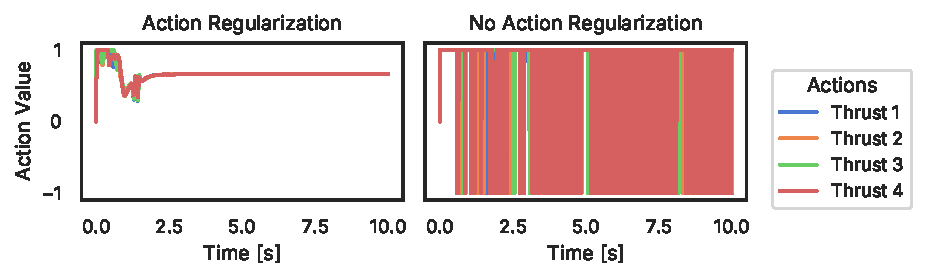
\includegraphics[width=\textwidth]{experiments/actions_comparison.pdf}
    \caption[Action Regularization]{Comparison of policy trained with and without the action regularization reward. The left plot shows the actions over time of the policy with regularization, while the right plot shows the actions of the policy without regularization. The regularized policy produces smoother and more stable actions, while the unregularized policy exhibits large fluctuations in thrust commands jumping between the action limits.}
    \label{fig:actions_comparison}  
\end{figure}
With high frequency continuous control tasks, we often observe that the policy learns to produce very aggressive actions, saturating the action range. To encourage smoother actions and reduce energy consumption, we introduce two regularization terms. One discourages actions at the limits of the action range, while the other penalizes large changes in rotor thrust and variations between rotors. Let \(\mathbf{a}_t^i,\mathbf{a}_{t-1}^i\) be consecutive normalized thrust vectors. The action smoothness reward is calculated as difference between consecutive actions and the mean thrust of the four rotors
\begin{equation}
r_{\rm smooth} = 20
\Biggl(
\frac{1}{Q}\sum_{i=1}^Q \bigl\lVert \mathbf{a}_t^i - \mathbf{a}_{t-1}^i \bigr\rVert_1
\;+\;
\frac{1}{Q}\sum_{i=1}^Q \bigl\lVert \mathbf{a}_t^i - \bar a_t^i\,\mathbf{1}\bigr\rVert_1
\Biggr), \quad \bar a_t^i = \frac{1}{4}\sum_{j=1}^4 a_{t,j}^i
\end{equation}

This term encourages smooth, low-frequency thrust commands and penalizes large changes in rotor thrust. Additionally we penalize actions that are close to the action limits, which can lead to aggressive behavior and instability. We define the energy cost as
\begin{equation}
r_{\mathrm{energy}} = \frac{1}{4Q}
\sum_{i=1}^{Q}\sum_{j=1}^{4}\exp\bigl(-50\,|a_{t,j}^i|\bigr)\;+\;\exp\bigl(50\,(a_{t,j}^i-1)\bigr)
\end{equation}

The first term discourages abrupt changes in thrust, while the second term penalizes high rotor speeds, which can lead to excessive energy consumption and instability. The exponential shaping ensures that the penalty is more pronounced for larger deviations, promoting smoother actions. 

Figure~\ref{fig:actions_comparison} shows the difference in actions between a policy trained with and without these two action regularization terms. The policy with regularization produces smoother and more stable actions, while the unregularized policy exhibits large fluctuations in thrust commands jumping between the action limits. This regularization is crucial for stable training and sim-to-real transfer.

\subsubsection{Aggregate Reward}
We combine the individual reward components into a single reward signal for each agent. The reward components for stability are grouped as
\begin{equation}
r_{\mathrm{stab}}
= \frac{1}{5}\bigl(r_{\mathrm{velP}} + r_{\mathrm{velQ}} + r_{\mathrm{yaw}} + r_{\mathrm{up}} + r_{\mathrm{taut}}\bigr)
\end{equation}
The safety components that should always be enforced are grouped as
\begin{equation}
r_{\mathrm{safety}}
= \frac{1}{5}\bigl(r_{\mathrm{coll}} + r_{\mathrm{oob}} + r_{\mathrm{smooth}} + r_{\mathrm{energy}} + r_{\mathrm{dist}}\bigr)
\end{equation}
Finally, we combine the tracking reward with the stability and safety components to form the overall reward
\begin{equation}
r
= r_{\mathrm{track}}\;r_{\mathrm{stab}}
\;+\;r_{\mathrm{safety}}.
\end{equation}
This product structure ensures the policy learns to track the payload while constantly maintaining stable formations. This is important because the simultaneous optimization of position error and velocities can lead to policies getting stuck in local minima, with a static payload position error remaining.
The additive safety penalties strictly discourage unsafe or aggressive behaviors.

This reward formulation naturally scales with the number of quadrotors \(Q\), retaining its structure and incentives as \(Q\) varies. It even works in the simplified case of a single quadrotor without a payload. We simply set \(r_{\mathrm{taut}}=1\) and use the quadrotor position for tracking error calculation. We still obtain a coherent reward that still encourages stable, smooth flight and graceful control even in the absence of cable-tautness considerations.

The reward structure can also be adapted to other tasks, by replacing the tracking reward component with other task-specific rewards. This makes the reward a good basis for a wide range of scenarios with multiple quadrotors. We can now apply our reward function to train policies for different numbers of quadrotors with and without payload.

% To train a policy for the quadrotor without a payload, we  set \(r_{\mathrm{taut}}=1\).
% % \subsection{Reward Design Considerations}
% \todo{write further reward design considerations}
% \subsection{Integration with JAXMARL}

% CrazyMARL integrates seamlessly with the JaxMARL ecosystem \cite{flair2023jaxmarl}.  We wrap each Brax environment in a \texttt{JAXMARL.Mabrax} adapter, exposing standard methods for rollout collection, batching, and replay buffer storage.  The same RL algorithms (e.g., PPO, QMIX) can be applied unchanged to single-agent or decentralized multi-agent tasks, enabling rapid experimentation across a broad class of cooperative aerial transport problems.

\todo{maybe consider adding a few lines about reward components that you considered but discarded in the final reward function}
\section{Training}
\begin{figure}[ht]
    \centering
    
    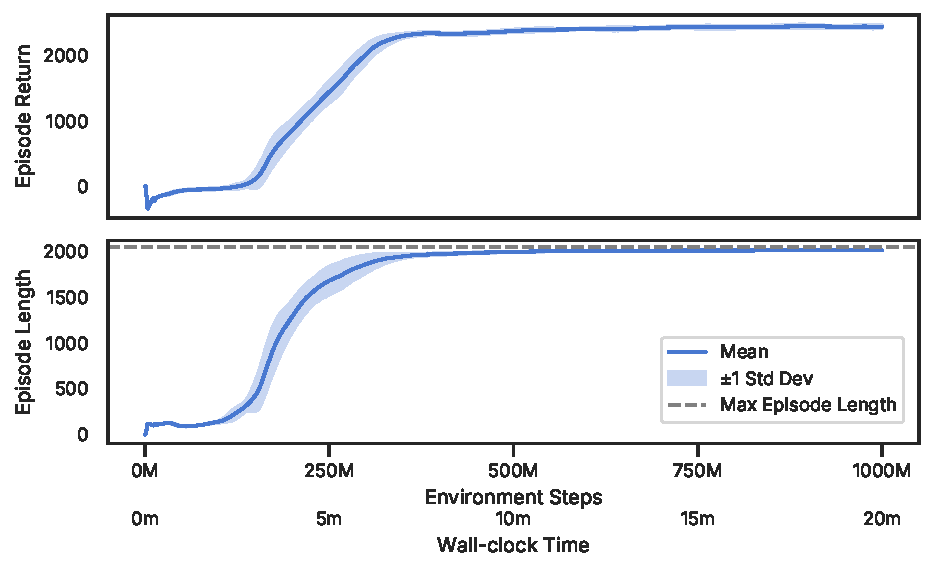
\includegraphics[width=\textwidth]{experiments/train_metrics.pdf}
    \caption[Training Metrics]{Average training metrics for one quadrotor with payload scenario. The top plot shows the average episode returns and the bottom plot shows the average episode lengths over environment steps and wall-clock time. The shaded area represents the standard deviation across 10 seeds. The maximum possible episode lenght here is 2048 environment steps, which corresponds to 8.2 seconds of flight time. In the end nearly all episodes are completing the episode indicating stable flight.}
    \label{fig:train_metrics}
\end{figure}
Our training pipeline follows the approach of \autocite{flair2023jaxmarl}, leveraging the JaxMARL framework as a basis to our training method. We use the \gls{ippo} algorithm, which extends \gls{ppo} to multi-agent settings by optimizing a joint policy across all agents while maintaining decentralized execution. We also investigated the use of \gls{mappo} wiht a centralized critic, but found that \gls{ippo} performs sufficient for few quadrotor scenarios.

The decentralized policies are learned end-to-end via \gls{ippo} within our highly parallelized JAX/MJX simulation environment. At each iteration, a fixed number of synchronous actors collect trajectories in $N$ parallel environments over $T$ time steps, yielding $NT$ experiences per update. Collected rewards are bootstrapped with the learned critic to compute targets, and advantages are estimated using \gls{gae} with discount factor $\gamma$ and smoothing parameter $\lambda$. The overall loss combines the clipped policy objective
\begin{equation}
L_{\mathrm{PPO}}(\theta) = \mathbb{E}\!\bigl[\min\bigl(r_t(\theta)\,\hat{A}_t,\;\mathrm{clip}(r_t(\theta),1-\epsilon,1+\epsilon)\,\hat{A}_t\bigr)\bigr],
\end{equation}
a mean-squared value-function error, and an entropy regularizer to encourage sufficient exploration. Gradient norms are clipped to enhance numerical stability.

Since our environment has a certain level of complexity we always train on a high number of parallel environments (16384). This might not be very sampling efficient but allows us to collect a large number of experiences with sufficient variance of configurations in a short time, which is crucial for stable training of policies. A lower number of environments also usually trains a working policy, but the training progress has higher varience and it is more likely to get stuck on local minima for position tracking. On each environment we only step 32 steps per episode. Giving us 128 Minibatches of size 4096 for each episode. The training is performed on a single GPU, which allows us to leverage the high-performance capabilities of JAX and Brax for efficient training. Figure~\ref{fig:train_metrics} shows the training progess of the two quadrotor policy. \todo{maybe add comparison of few env traing to fig}

The training process and hyperparameters are virtually the same for all number of quadrotors, only the policy size is slightly adjusted for more quadrotors. We train the policy on a single RTX Ada 4000 GPU with 20GB of RAM. This gives us training speeds of up to 1 Million environment steps per second, depending on the number of parallel environments and Quadrotors. We trained the policies in our experiments on one Billion environment steps, which corresponds to roughly 10 minutes of training time for the single quadrotor task and 20 minutes for the dual quadrotor task and 60 minutes for the three quadrotor tasks. We are also able to train a single quadotor policy without payload in less than 3 minutes.

\subsection{Policy Architecture}
Both actor and critic networks are instantiated as fully connected, feed-forward multilayer perceptrons. The actor network comprises an input layer matching the local observation dimension, three hidden layers of 64 units with tanh activations, and a linear output layer producing the action-mean vector. A learned log-standard deviation vector of the same dimensionality parameterizes a diagonal Gaussian policy. The critic network features three hidden layers of 128 tanh units each, terminating in a scalar output. All dense layers employ orthogonal weight initialization and zero biases. During training and rollouts, actions are sampled stochastically from the policy distribution, at evaluation time, the deterministic mean action is used.

\subsection{Hyperparameters}
We run a Bayesian optimization sweep, with early termination of runs, over the hyperparameters to find the best configuration for our task. We first conduct a coarse search over a wide range of values, then refine the search around the most promising regions. The final hyperparameters are selected based on the best performing policy with the highest reward. Table~\ref{tab:hyperparams} summarizes the key hyperparameters used in our experiments.

\begin{table}[ht]
  \centering
  \caption{Key hyperparameters for training.}
  \label{tab:hyperparams}
  \begin{tabular}{@{}ll@{}}
    \toprule
    Hyperparameter & Value \\
    \midrule
    Total environment timesteps    & $1\times10^{9}$ \\
    Number of environments & 16,384 \\
    Number of steps per update & 32 \\
    Number of minibatches & 128 \\
    Update epochs & 8 \\
    Anneal learning rate & false \\
    Learning rate & $4\times10^{-4}$ \\
    Activation function & \texttt{tanh} \\
    Entropy coefficient & 0.01 \\
    Discount factor ($\gamma$) & 0.995 \\
    \gls{gae} lambda ($\lambda$) & 0.95 \\

    Actor network architecture & [64, 64, 64] \\
    Critic network architecture & [128, 128, 128] \\
    \bottomrule
  \end{tabular}
\end{table}



